% 例 3：以 O（△ABC 内部一点）为位似中心、k=1/2 作 △A'B'C'
\documentclass[tikz,border=4pt]{standalone}
\usepackage{ctex}
\usepackage{amsmath}
\usetikzlibrary{calc, arrows.meta}
\begin{document}
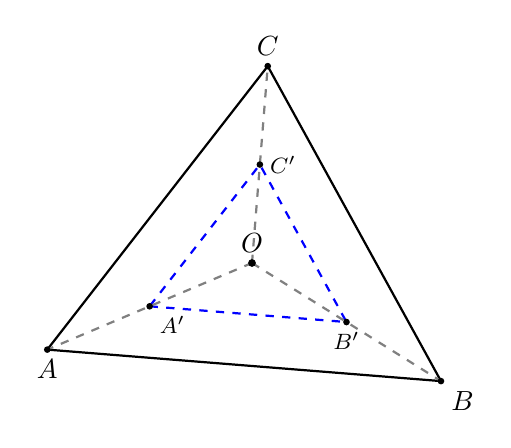
\begin{tikzpicture}[scale=1.0, thick]
  \coordinate (A) at (-2.4, -1.2);
  \coordinate (B) at (2.6, -1.6);
  \coordinate (C) at (0.4, 2.4);
  \coordinate (O) at (0.2, -0.1);
  % A' = O + 0.5*(A-O)
  \coordinate (Ap) at ($(O)!0.5!(A)$);
  \coordinate (Bp) at ($(O)!0.5!(B)$);
  \coordinate (Cp) at ($(O)!0.5!(C)$);

  \draw (A) -- (B) -- (C) -- cycle;
  \draw[blue, dashed] (Ap) -- (Bp) -- (Cp) -- cycle;
  \draw[gray, dashed] (O) -- (A);
  \draw[gray, dashed] (O) -- (B);
  \draw[gray, dashed] (O) -- (C);

  \fill (O) circle (1.4pt);
  \fill (A) circle (1.2pt); \fill (B) circle (1.2pt); \fill (C) circle (1.2pt);
  \fill (Ap) circle (1.2pt); \fill (Bp) circle (1.2pt); \fill (Cp) circle (1.2pt);
  \node[below] at (A) {$A$};
  \node[below right] at (B) {$B$};
  \node[above] at (C) {$C$};
  \node[above] at (O) {$O$};
  \node[below right] at (Ap) {\footnotesize $A'$};
  \node[below] at (Bp) {\footnotesize $B'$};
  \node[right] at (Cp) {\footnotesize $C'$};
\end{tikzpicture}
\end{document}
